
\documentclass[11pt,twocolumn]{article}

\usepackage[paperheight=297mm,paperwidth=210mm,top=25mm,bottom=25mm,left=25mm,right=25mm]{geometry}

\usepackage{txfonts}
\usepackage{graphicx}
\usepackage[T1]{fontenc}
\usepackage[icelandic]{babel}
\usepackage{listings}
\usepackage[utf8]{inputenc}
\usepackage[bf]{caption}
\graphicspath{{./}}


\setlength{\baselineskip}{0pt} 
\setlength{\parindent}{0pt}
\setlength{\parskip}{0pt}

\usepackage{graphicx}
\title{ Heimadæmi 5 - Tölvugrafík }
\date{}

\author{Davíð Isebarn Ágústsson }
\begin{document}
\maketitle

\section*{Dæmi 1}

https://notendur.hi.is/~dia2/203M/HD/HD5/

\section*{Dæmi 2}
Ef við hefðum eftirfarandi punkta:
a [-0.5,0.5,0.0] 
b [-0.5,-0.5,0.0]
c [0.5,-0.5,0.0]
d [0.5,-0.5,0.0]

þ.a 


\includegraphics[width = \linewidth]{9.png}

Þá gæti ég fyllt uppí bæði með TRIANGLE$\_$FAN eða TRIANGLE$\_$STRIP

TRIANGLE$\_$FAN 
Fyrsti punkturinn sem fer inní TRIANGLE$\_$FAN er "miðpunkturinn" 
og verður einn punktanna í öllum þríhyrningum sem verða teiknaðir
Til að mynda fyrsta þríhyrninginn þá þarf miðpunktinn og síðan punkt
2 og punkt 3. 

Næsti þríhyrningur þar á eftir notar miðpunktinn,
punkt 3 og nýja punktin, punkt 4. 

Þriðji þríhyrningurinn myndi nota miðpunktinn,
punkt 4 og nýja punktinn, punkt 5

Til að fylla upp í ferhyrninginn með punktum a,b,c,d þá gætum við
sett inn í TRIANGLE$\_$FAN í eftirfarandi röð:
a,b,d,c
Þá teiknast fyrst þríhyrningur með punkta a,b,d
Síðan þríhyrningur með a,d,c


TRIANGLE$\_$STRIP
TRIANGLE$\_$FAN notar alltaf sama miðpunktinn, elsta punktinn og 
nýja punktinn
TRIANGLE$\_$STRIP notar elsta, næstelsta punktinn og nýjasta 
punktin
Þá myndum við kalla á TRIANGLE$\_$STRIP með:
a, b, a, d, c

Þá búum við fyrst til "ósýnilegann" þríhyrning með 
punktanna a,b,a
Síðan þríhyrning með punktanna b,a,d
Seinast með punktunum a,d,c

\newpage

\



\section*{Dæmi 3}

Stuðlarnir I og k eru báðir vigrar. I eru litir ljósgjafa og k eru litir yfirborðs, ka er ambient litur yfirborðs, kd er diffuse litur yfirborðs og ks er specular litur yfirborðs
Vigrarnir geyma gildin r,g,b,a, öll frá 0-1

Þetta er samt frekar ambiguous spurning, en bókin gefur til kynna að stuðlarnir ka, kd og ks séu skalarstærðir frá 0-1 og segir síðan beint á eftir að þeir séu liðaðir í r,g,b,a 


\newpage

\

\newpage

\

\section*{Dæmi 4}

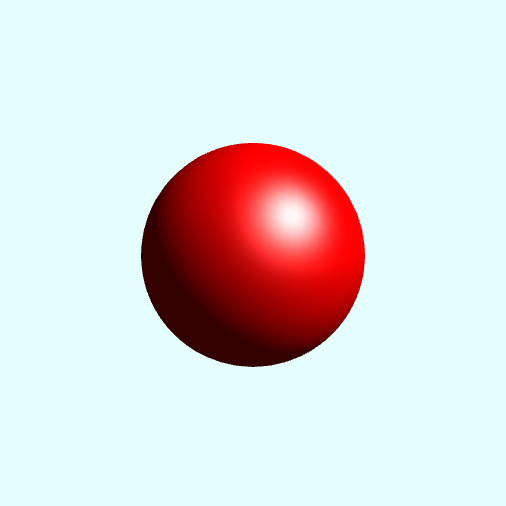
\includegraphics[width = 0.45\linewidth]{1.png}
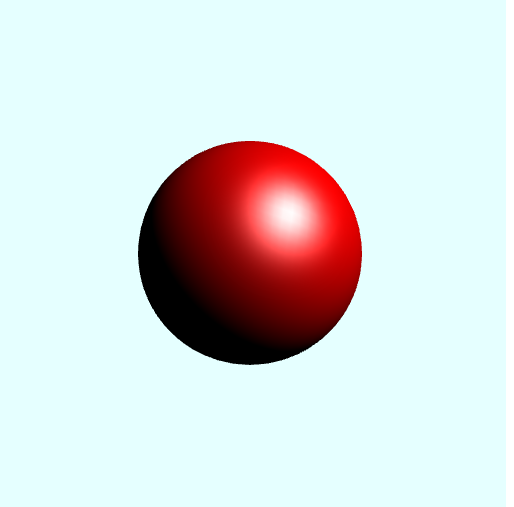
\includegraphics[width = 0.45\linewidth]{2.png}

Á myndunum er fyrri myndin með ambient-lið í bútalitaranum (fragment-shader) en í seinni myndinni hef ég tekið hann út

Munurinn er að ef ambient-lið vantar þá verða óupplýstir hlutar myndarinnar kolsvartir sem er óraunverulegt nema þegar það á að vera ekkert umhverfi sem ljós varpast af, eins og í geimnum


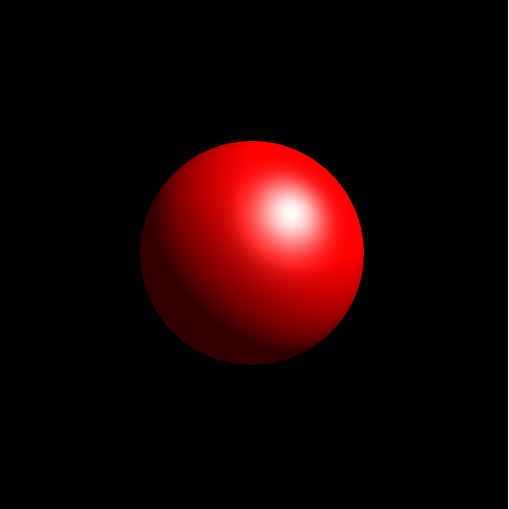
\includegraphics[width = 0.45\linewidth]{3.png}
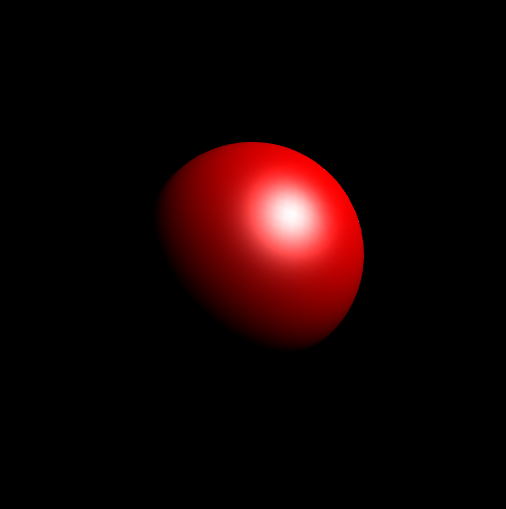
\includegraphics[width = 0.45\linewidth]{4.png}

Á þessum myndum  höfum við rauðu kúluna "í geimnum" með ambient-lýsingu  en þá lýtur það augljóslega undarlega út en á mynd 4 er slökkt á ambient-lýsingunni og þá kemur það mjög eðlilega út og auðvelt að sjá að umhverfisendurskyn  vantar, því hér á það að vanta en eini teljandi ljósgjafinn væri sólin


\newpage

\

\newpage

\

\section*{Dæmi 5}

\subsection*{a-liður}

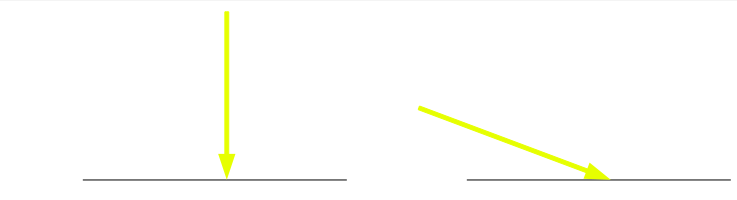
\includegraphics[width = \linewidth]{5.png}

Diffuse lýsing lýsir mest upp þá hluti sem snúa að ljósgjafanum, þ.e.a.s ef að ljósgjafi lýsir beint niður á hlut (undir $0^{\circ}$ horni) þá lýsist hluturinn 'fullkomnlega' upp, en því hærra sem hornið verður því minni verður lýsingin

Því verður sá hluti sem er beint undir ljósgjafanum bjartastur í augum áhorfenda, almennt þeir fletir sem snúa beint að ljósgjafanum eru þeir sem lýsast mest

Þetta kemur til vegna þess að diffuse lýsingin fylgir lögmáli \textbf{Lambert} sem segir að endurskinið, R (það sem áhorfandi sér) er í réttu hlutfalli við $\cos\theta$ 

\[
R \propto \cos\theta
\]

þar sem $\theta$ er hornið sem ljósgjafinn myndar við normalvigur flatarins sem það skellur á

\subsection*{b-liður}

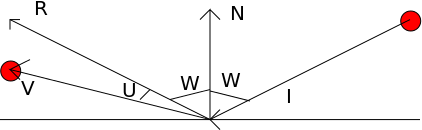
\includegraphics[width = \linewidth]{D5A.png}

  Ef að N er normalvigurinn frá yfirborðinu og I er vigur ljósgjafans þá er  W hornið á milli N og I
  Hámarks endurskin verður eftir vigrinum R sem myndar hornið 2W við I

  Ef að V er vigurinn frá punktinum sem ljósgjafinn lendir á yfirborðinu að auganum, þá er U hornið sem er á milli endurskinsvigursins R og vigurs augans V

  Á myndinni sést ljósgjafi sem er tvöfalt hærra yfir yfirborðinu en áhorfandinn, og skýn á yfirborðið mitt á milli þeirra

  Þá verður hámarksendurskin fyrir áhorfenda sem er staddur í R en því stærra sem hornið U verður því minna verður endurskynið

Þá þurfum við að breyta punktinum sem ljósgjafinn lýsir á, til þess að koma áhorfendanum akkúrat inní R:

Ef að:
\begin{itemize}
\item $d$ er fjarlægð frá miðpunkti ljósgjafa og athuganda á x-ásinum
\item $a$ er einhver óþekkt fjarlægð á x-ás
\item $h$ er hæð yfir x-ás
\item $\theta$ er hornið sem ljósvigurinn myndar við normalvigurinn
\item $\alpha$ er hornið milli athuganda og endurspeglunarvigursins
\end{itemize}

þá viljum við finna $a$ í jöfnunni

\[
90 - \tan^{-1}\bigg(\frac{2h}{d+a}\bigg) = 90 + \alpha - \tan^{-1}\bigg(\frac{h}{d-a}\bigg)
\]

sem fæst með útleiðslu útfrá myndinni

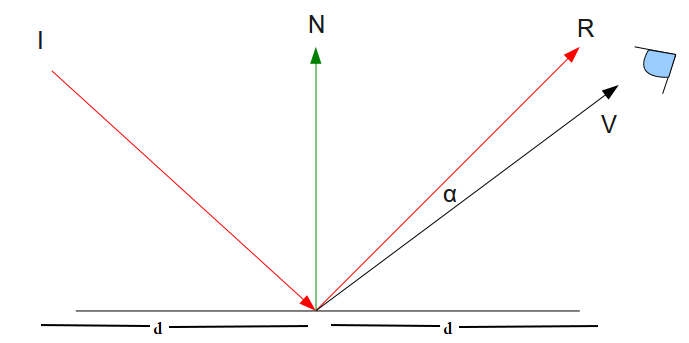
\includegraphics[width = \linewidth]{6.png}


og með nokkrum skrefum einfaldast jafnan í

\[
d = 3a \to a = \frac{d}{3}
\]

sem þýðir að ef að athugandi er í punktinum $-d$ m.v x-ás og ljósgjafinn í punktinum $d$ m.v x-ás, þá er 0 mitt á milli þeirra, og hámarksspeglunin verður í punktinum $a = \frac{d}{3}$

\subsection*{c-liður}

Diffuse endurskyn myndi ekkert breytast en það er ekki háð staðsetningu athugandans, heldur einungis staðsetningu ljóssins og afstöðu hvers flatar við ljósgjafann

Specular lýsingin er þó ekki eins en þar er hámarks ljósafl mitt á milli athuganda og ljósgjafa ef flöturinn er þvert á ljósgjafann, en jafna fyrir styrkleika specular-liðsins er 

\[
Specular \times (Half \dot Normal)^n
\]

þar sem

\[
Halft = \frac{Light+View}{||Light + View||}
\]

sbr við mynd

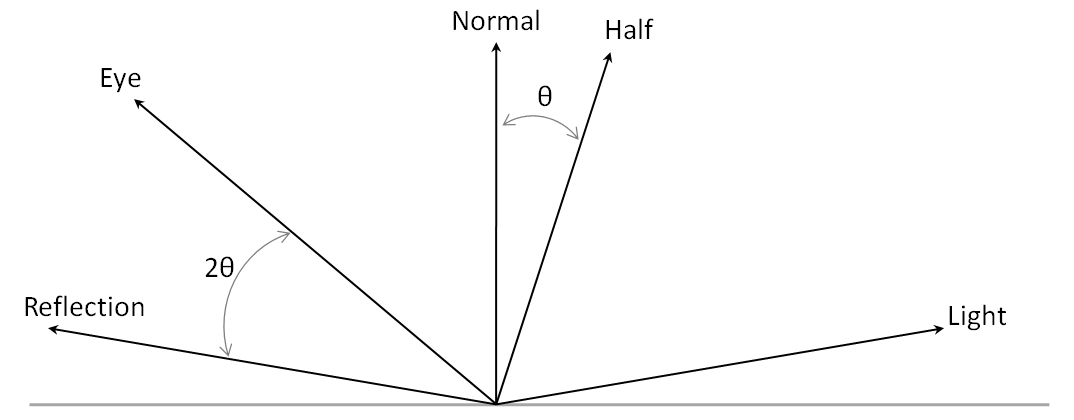
\includegraphics[width = \linewidth]{7.png}

en ljóst er að hámarksendurskyn er mjög háð $Normal$ vigrinum (sbr við fyrri jöfnuna) en $Normal = (0,1,0)$ svo hér höfum við einungis $y$-lið til að margfalda uppúr depilmargfeldinu, svo að við þurfum að sjá til þess að $y$-liður $Half$ vigursins sé eins stór og hægt er, en því stærri sem $x$ eða $z$ liðirnir eru, því meira erum við að troða ofaní nefnarann í seinni jöfnunni, sem minnkar teljarann, án þess að $x$ og $z$ liðirnir séu að bæta einhverju við til að stækka $Half \dot Normal$ depilmargfeldið

Því er ljóst að við fáum út (sbr við b-lið) að mest fæst ef að $a = 0$ og að staðsetning athuganda sé í $-d$ og staðsetning ljósgjafa sé $d$ en þá styttast þeir liðir út í jöfnunni fyrir $Half$ og þá fáum við hæsta gildið, sem er mitt á milli þeirra, í $0$ punktinum m.v x-ás

\end{document}